\chapter{Orderbook Trading Simulator}
\label{chap:simulator}
This chapter describes the \ac{OTS} and it's underlying OrderbookContainers, implemented within the scope of this thesis. Fed with historic orderbook data it serves as a backtesting framework for testing out various trading strategies. The \ac{OTS} provides detailed feedback in terms of trading progress, achieved prices and accrued costs.

\section{Data Origin}
Since typical financial data providers must make an earning from their treasures, they typically only deliver delayed market data on a complimentary basis. Investors dependent on real time or level 2 market data (see \Cref{sec:marketdata:levels}) are usually charged horrendous monthly subscription fees.\\

A costless alternative exists in open cryptocurrencies, like bitcoins (see \Cref{chap:bitcoins}). The digital asset exchange platform Poloniex \cite{poloniex} provides an open API for querying detailed market data in real time. As their push API, to receive live order book updates and trades, was rather error-prone and buggy when this project started, the decision was made, to query full orderbooks on a minutely basis. Via HTTP GET requests, Poloniex delivers orderbook snapshots up to a market depth of 5000 bids and asks. The volume of recorded orderbook snapshots for nine distinct currency pairs\footnote{Recorded currency pairs include USDT/BTC, BTC/ETH, BT/XMR, BTC/XRP, BTC/FCT, BTC/NAV, BTC/DASH, BTC/MAID, BTC/ZEC} since Nov, 10th 2016 amounts to roughly 100GB (as per 2017-06-20). This thesis concentrates on the currency pair USDT/Bitcoin.

\begin{lstlisting}[frame=single, breaklines=true, basicstyle=\scriptsize, caption=Data fetched from Poloniex via HTTP GET request, label=lst:PoloniexFetch]
# https://poloniex.com/public?command=returnOrderBook&currencyPair=USDT_BTC&depth=5000
{"asks" :[[ "705.450000" ,2.772181], [ "705.450196", 0.139212] ,["706.170000" ,0.052838] , ... ], "bids":[["705.000000",0.158232],["703.700000" ,0.001250], ... ], "isFrozen": 0, "seq": 63413296}
\end{lstlisting}

\begin{figure}[ht]
	\centering
   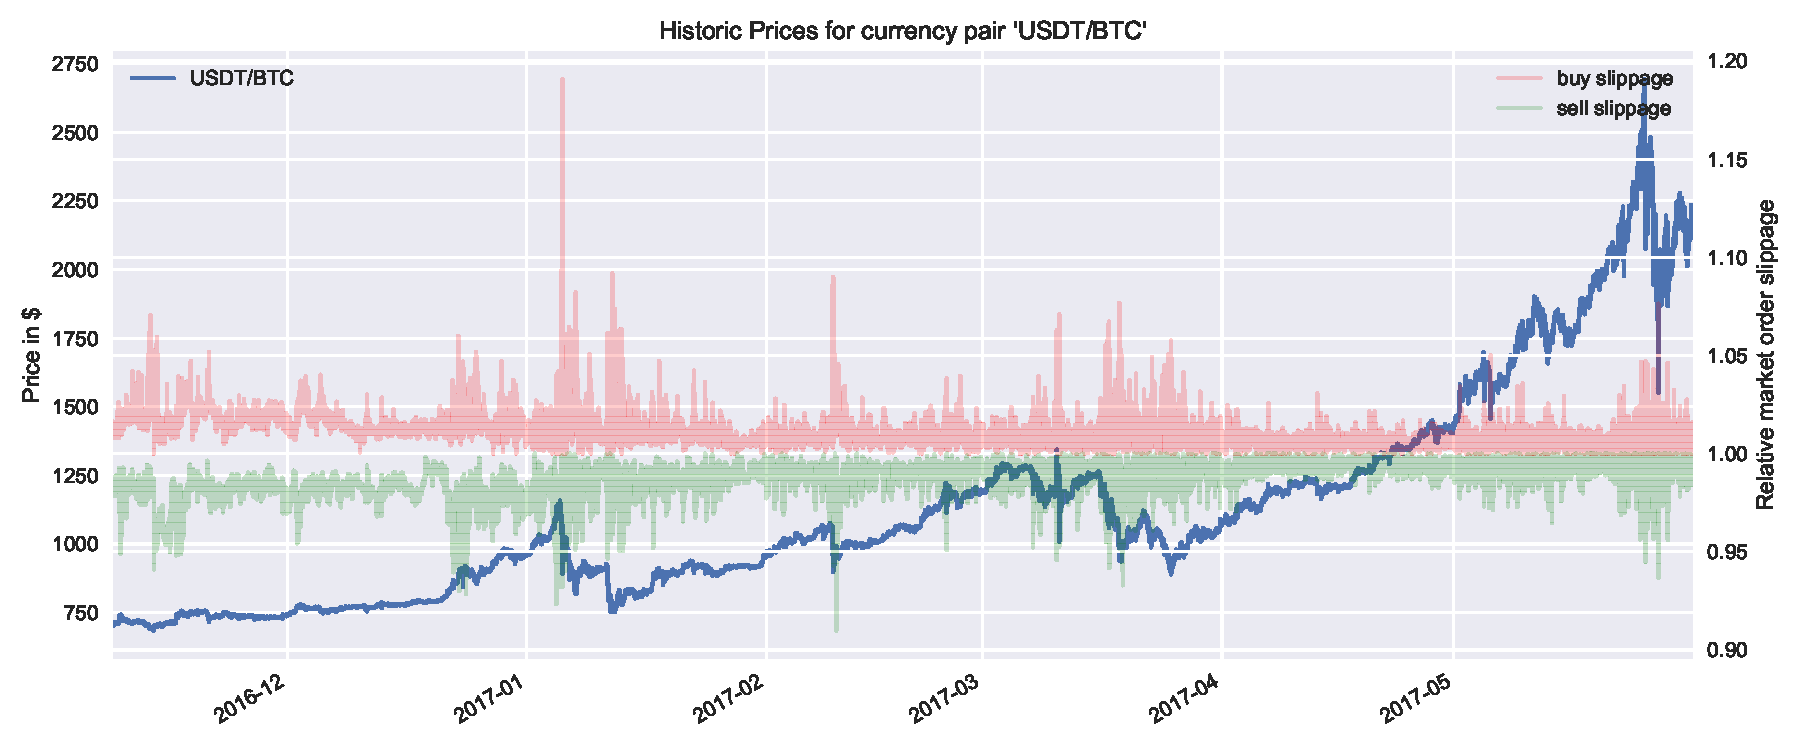
\includegraphics[width=0.4\textwidth]{content/drawings/bitcoin_historicPrices}
	\caption{Historic center prices between Nov, 10th 2016 and Mar, 31 2017, as fetched from Poloniex)}
	\label{fig:ploniexPriceHistory}
\end{figure}

\section{Data preprocessing}
The python \lstinline!class OrderbookContainer! aggregates all informations contained in an individual orderbook snapshot. It enforces correct price ordering in the two opposing bid and ask books and provides additional methods for market visualization and feature extraction. To restrict wasteful memory usage, orderbook snapshots are condensed in two ways:

\begin{itemize}
\item Almost identically price levels are round to the second decimal and their respective order volumes merged.

 \[ 
  \begin{rcases}
    0.139212 * 705.450000\\
    2.632969 * 705.450196\\
  \end{rcases} 
  = 2.772181 * 705.45
\]
\item Market depth is capped just above the threshold of 100 bitcoins, roughly corresponding to a market depth of 100-140 prices levels in both books. This threshold allows to simulate trades up to a market order price of 70.000 \$ at any time throughout the whole recording period.

\end{itemize}

\Cref{lst:OrderbookContainer} shows the most important functions, provided by the OrderbookContainer class. OrderbookContainer Instances are vigorously used by the \ac{OTS}.

\begin{lstlisting}[frame=single, breaklines=true, basicstyle=\scriptsize, caption=OrderbookContainer, label=lst:OrderbookContainer]
ob = OrderbookContainer(timestamp="2016-11-08T10:00",
                        bids=pd.DataFrame([200., 100., 300.],
                        columns=['Amount'], index=[28.7, 28.5, 28]),
                        asks=pd.DataFrame([25., 50., 200.],
                        columns=['Amount'], index=[29., 30., 31.]))
# Available methods
ob.plot(outfile='sample.pdf')  # plt.show or plt.savefig
ob.asks  # pd.DataFrame
ob.bids  # pd.DataFrame
ob.features  # returns a dict of precomputed features
ob.get_bid(), ob.get_ask(), ob.get_center()  # float
ob.get_current_price(volume=100)  # float
ob.get_current_sharecount(cash=70000) # float
ob.compare_with(other_ob) # returns orderbook deltas used by the OTS
ob.enrich()  # computes Volume, VolumeAcc and norm_Price
ob.head(depth=3)  # caps orderbook at a market depth of 3
ob.plot()
\end{lstlisting}


\begin{figure}[ht]
	\centering
   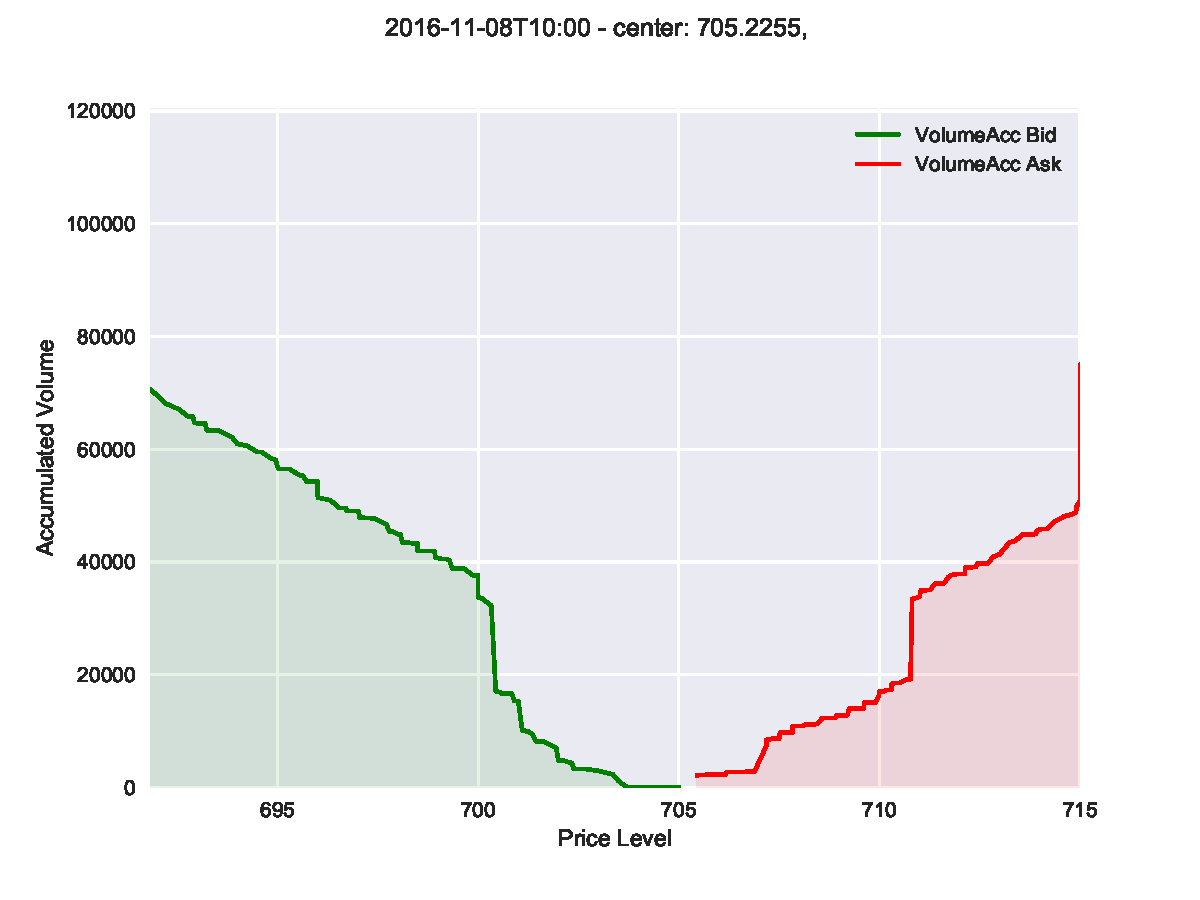
\includegraphics[width=0.9\textwidth]{content/drawings/orderbook.jpg}
	\caption{Episode Window over 120 minutes (increasing prices)}
	\label{fig:orderbook}
\end{figure}


\section{Simulator}
bla

\section{Evaluation / Comparison of strategies}
bla

\cleardoublepage{}